% Provenance (never printed): see sources/outline_sources.md (Year 1: vertical structure of
% the atmosphere, lapse rates, potential temperature and static stability; the layered
% ocean, the equation of state of seawater, T-S diagrams and water masses). Exercise and
% problem values in the Book 3 scratch calculator calc/ch26.py; figures from
% figdata/bachelor-1/atmosphere_profile.py (U.S. Standard Atmosphere 1976) and
% seawater_eos.py (EOS-80 and the UNESCO 44 algorithms; WOA23 columns, datasets
% bachelor-1-woa23-* and Book 2's grade-10-woa23-arctic-*).
% Physics owns the hydrostatic relation, the isothermal atmosphere and its scale height,
% the first law, Laplace's relation and Archimedes' thrust (recalled). Book 1 (g8) gave
% the layers and the environmental lapse rate of 6.5 K/km; Book 2 (g10) the dry adiabatic
% rate admitted, stable and unstable air, the mixed layer, thermocline, halocline and
% pycnocline: re-founded here with derivations. The moist adiabat is the Year 2 volume's.
\chapter{بنية الغلاف الجوي والمحيط}\label{ch:b1:fluid-envelopes-structure}

مرّتين في اليوم، في محطات الأرصاد حول العالم، يُطلَق بالون يحمل جهازًا صغيرًا للإرسال اللاسلكي (مسبار راديوي)، يُرسل قراءات الضغط ودرجة الحرارة والرطوبة في الهواء وهو يصعد؛ فيتسلّق بنحو \qty{300}{m} في الدقيقة، ويمكن أن يبلغ \qty{35}{km} قبل أن ينفجر البالون. وفي عرض البحر، تُنزل سفينة بحث إطارًا من الأجهزة وزجاجات الماء بكابل نحو الهاوية، فتقيس الموصلية والحرارة والعمق طوال الطريق. والمقطعان، أحدهما للهواء والآخر للماء، هما المادة الخام لهذا الفصل. والغلافان طبقيّان كلاهما، والطبقية فيهما تحدّدها الكثافة: سائل خفيف فوق سائل ثقيل. وما يجعل طبقة خفيفة أو ثقيلة أقلّ وضوحًا مما يبدو: فالهواء الأبرد من الهواء الذي تحته قد يظلّ الأخفّ؛ والماء الأدفأ من الماء فوقه قد يظلّ الأثقل. ويبني الفصل أداتين تفرزان ذلك، هما \omterm{def:b1:fluid-envelopes-structure:potential-temperature}{درجة الحرارة الكامنة} \omterm{def:b1:fluid-envelopes-structure:eos}{ومعادلة حالة ماء البحر}.
% ledger: nws:radiosonde, nws:radiosonde-def, commons:ctd-rosette

\begin{omfigure}
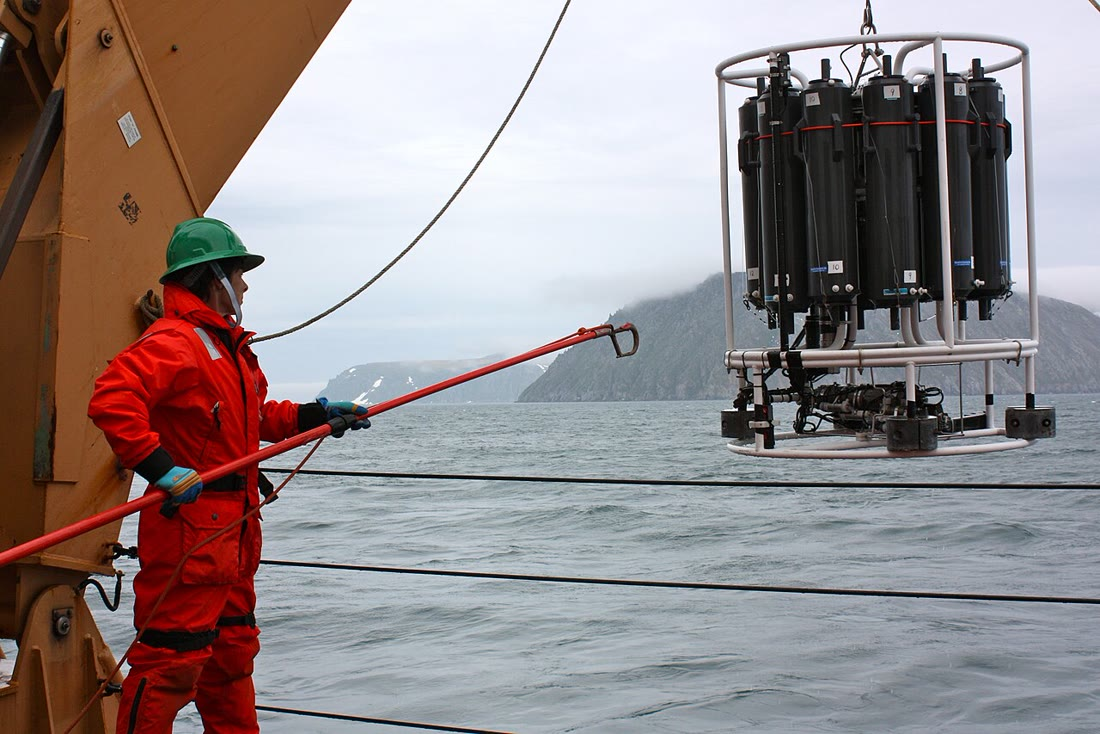
\includegraphics[width=0.62\linewidth]{images/book3/b1-ctd-rosette.jpg}

{\small جهاز CTD وإطار الزجاجات (rosette) يُعادان إلى ظهر السفينة في مضيق بيرينغ في يونيو 2011. والزجاجات الرمادية حول الإطار تُغلق على أعماق مختارة أثناء الصعود لأخذ عيّنات الماء؛ والأجهزة في أسفل الإطار تقيس الموصلية (التي تُحسب منها الملوحة)، والحرارة، والعمق (في الحقيقة الضغط) باستمرار أثناء إنزال الإطار. (NASA Goddard Space Flight Center, ملك عام، عبر Wikimedia Commons.)}
\label{fig:b1:fluid-envelopes-structure:ctd}
\end{omfigure}
% ledger: commons:ctd-rosette, unesco44:atg-theta

\begin{recall}
تُعطي الكتب الفيزيائية العلاقة الهيدروستاتيكية، $\mathrm dp/\mathrm dz =
-\rho g$، لسائل ساكن؛ ولغاز مثالي كتلته المولارية $M$، $p = \rho R
T/M$، وفي غلاف جوي متساوي الحرارة ينخفض الضغط ك$e^{-z/H}$ مع ارتفاع المقياس $H = RT/(Mg)$. وتصوغ القانون الأول للحرارة لنظام مغلق، وبالنسبة إلى غاز مثالي، علاقة لابلاس على طول تحوّل أديباتي عكوس، $pV^{\gamma} = $ ثابت، مع $\gamma = c_p/c_v$ و$c_p - c_v
= R/M$ لكل وحدة كتلة. ويتلقّى جسم مغمور في مائع دفعًا لأعلى يساوي وزن المائع الذي يزيحه (أرخميدس). وسمّى الكتاب الأول طبقات الغلاف الجوي \omterm{def:b1:fluid-envelopes-structure:lapse-rate}{ومعدّل الانخفاض البيئي} للغلاف الجوي المعياري، \qty{6.5}{\celsius} لكل كيلومتر في التروبوسفير؛ وأقرّ الكتاب الثاني \omterm{def:b1:fluid-envelopes-structure:lapse-rate}{معدّل الانخفاض الأديباتي الجاف}، \qty{9.8}{\celsius} لكل كيلومتر، ووصف الهواء بأنه مستقرّ أو غير مستقرّ بحسب مصير طرد يُدفع إلى أعلى، ووصف \omterm{def:b1:fluid-envelopes-structure:ocean-layers}{الطبقة المختلطة}، \omterm{def:b1:fluid-envelopes-structure:ocean-layers}{والترموكلاين}، \omterm{def:b1:fluid-envelopes-structure:ocean-layers}{والهالوكلاين} \omterm{def:b1:fluid-envelopes-structure:ocean-layers}{والبيكنوكلاين} للمحيط. وماء البحر قريب من 35 غرامًا من الأملاح المذابة لكل كيلوغرام.
% ledger: ussa76:layers, nws:dalr, nos:salinity
\end{recall}

\section{البنية الرأسية للغلاف الجوي}\label{sec:b1:fluid-envelopes-structure:atmosphere}

لا يشبه أيّ مسبار حقيقي التالي. وللمقارنة يُثبَّت مقطع مرجعي بالاتفاق.

\begin{definition}[الغلاف الجوي المعياري]\label{def:b1:fluid-envelopes-structure:standard-atmosphere}
\emph{الغلاف الجوي المعياري}\index{الغلاف الجوي المعياري} مقطع للحرارة والضغط والكثافة بدلالة الارتفاع، مُثبَّت بالاتفاق: هواء جاف ثابت الكتلة المولارية، غاز مثالي في توازن هيدروستاتيكي، بقيم معطاة عند مستوى البحر، وحرارة تتغيّر خطّيًّا مع الارتفاع في طبقات متتالية. ويأخذ المعياري 1976 القيم \qty{288.15}{K} و\qty{101325}{Pa} عند مستوى البحر، و$M_0 = \qty{28.9644}{kg.kmol^{-1}}$،
$R^* = \qty{8314.32}{J.kmol^{-1}.K^{-1}}$ و$g_0 = \qty{9.80665}{m.s^{-2}}$.
\end{definition}
% ledger: ussa76:sea-level

أسفل \qty{47}{km} يملك المعياري 1976 أربع طبقات (\cref{tab:b1:fluid-envelopes-structure:layers}). والأدنى، التروبوسفير، يبرد ب\qty{6.5}{K} لكل كيلومتر؛ ومن قمّته، التروبوبوز، تبقى الحرارة عند \qty{216.65}{K} لتسعة كيلومترات، ثم ترتفع. وارتفاعات المعياري هي ارتفاعات جيوبوتنشيالية، أي الارتفاعات التي يعطي فيها جاذبية ثابتة $g_0$ الطاقة الكامنة نفسها؛ وأسفل \qty{32}{km} تختلف عن الارتفاعات الهندسية بأقلّ من \qty{0.6}{\percent} (\qty{11}{km} من المعياري تقع عند \qty{11.02}{km}).
% ledger: ussa76:layers, ussa76:sea-level

\begin{table}[ht]
\centering
\small
\renewcommand{\arraystretch}{1.2}
\begin{tabular}{|l|c|c|c|c|}
\hline
الطبقة & القاعدة (km) & $\mathrm dT/\mathrm dz$ (K/km) & $T$ عند القاعدة (K) & $p$ عند القاعدة (hPa) \\
\hline
1 (التروبوسفير) & 0 & $-6.5$ & 288.15 & 1013.25 \\
2 (الستراتوسفير) & 11 & 0.0 & 216.65 & 226.32 \\
3 (الستراتوسفير) & 20 & $+1.0$ & 216.65 & 54.75 \\
4 (الستراتوسفير) & 32 & $+2.8$ & 228.65 & 8.68 \\
\hline
\end{tabular}
\caption{الطبقات الأربع الدنيا للمعياري 1976 \omterm{def:b1:fluid-envelopes-structure:standard-atmosphere}{الغلاف الجوي المعياري}. والتدرّجات وقيم مستوى البحر هي قيم تعريفية؛ أما الحرارات والضغوط عند القواعد فتُحسب منها ب\cref{prop:b1:fluid-envelopes-structure:layer-pressure}.}
\label{tab:b1:fluid-envelopes-structure:layers}
\end{table}
% ledger: ussa76:layers, ussa76:sea-level (bases computed in figdata/bachelor-1/atmosphere_profile.py)

في كل طبقة تكون الحرارة دالة خطّية للارتفاع، فيمكن تكامل العلاقة الهيدروستاتيكية في صيغة مغلقة.

\begin{proposition}[الضغط في طبقة ذات تدرّج ثابت]\label{prop:b1:fluid-envelopes-structure:layer-pressure}
في طبقة من الهواء الجاف حيث $T = T_b - L\,(z - z_b)$ مع $L \neq 0$ ثابتًا، يكون الضغط
\[
  p = p_b \left(\frac{T}{T_b}\right)^{gM/(RL)},
\]
حيث $T_b$ و$p_b$ هما القيمتان عند القاعدة $z_b$. وحين يكون $L = 0$ ينخفض الضغط أسّيًّا مع ارتفاع المقياس $H = RT_b/(Mg)$.
\end{proposition}

\begin{proof}
تعطي العلاقة الهيدروستاتيكية والغاز المثالي $\mathrm dp/p = -(gM/R)\,\mathrm
dz/T$. وبما أن $\mathrm dT = -L\,\mathrm dz$، فهذا يصير $\mathrm dp/p =
(gM/(RL))\,\mathrm dT/T$، الذي يتكامل إلى $\ln(p/p_b) = (gM/(RL))
\ln(T/T_b)$. وحين يكون $L = 0$، فإن $T = T_b$ و$\ln(p/p_b) = -(z - z_b)/H$: الغلاف الجوي متساوي الحرارة من كتب الفيزياء.
\end{proof}

في تروبوسفير المعياري، $gM/(RL) = 9.80665 \times 28.9644 /
(8314.32 \times 0.0065) = 5.256$، وعند \qty{11}{km}، $T = 216.65$~K:
$p = \num{101325} \times (216.65/288.15)^{5.256} = \qty{22632}{Pa}$، أي أقلّ قليلًا من ربع قيمة مستوى البحر. وفي الطبقة متساوية الحرارة فوقها، $H =
8314.32 \times 216.65/(28.9644 \times 9.80665) = \qty{6.34}{km}$، وبعد تسعة كيلومترات أعلى ينخفض الضغط بعامل إضافي $e^{9/6.34} =
4.13$، إلى \qty{5475}{Pa}. وبما أن الضغط عند مستوى هو وزن الهواء فوقه لكل وحدة مساحة، فنصف كتلة المعياري يقع أسفل \qty{5.5}{km} وتسعة أعشارها أسفل \qty{16}{km}.
% ledger: ussa76:sea-level, ussa76:layers (values computed in figdata/bachelor-1/atmosphere_profile.py)

\section{معدّلات الانخفاض ودرجة الحرارة الكامنة}\label{sec:b1:fluid-envelopes-structure:lapse}

\begin{definition}[معدّلات الانخفاض البيئي والأديباتي الجاف]\label{def:b1:fluid-envelopes-structure:lapse-rate}
\emph{معدّل الانخفاض البيئي}\index{معدّل الانخفاض البيئي} هو $\Gamma =
-\mathrm dT/\mathrm dz$، معدّل انخفاض حرارة الهواء الساكن مع الارتفاع، كما يقيسه المسبار. و\emph{معدّل الانخفاض الأديباتي الجاف}\index{معدّل الانخفاض الأديباتي الجاف} $\Gamma_d$ هو معدّل انخفاض حرارة طرد من الهواء غير المشبع حين يُرفع.
\end{definition}
% ledger: nws:dalr

معدّل الانخفاض موجب حين تنخفض الحرارة مع الارتفاع. والمعدّلان من طبيعتين مختلفتين: الأول يصف حالة الغلاف الجوي في لحظة واحدة؛ والثاني يصف تحوّل قطعة من الهواء تتحرّك.

\begin{definition}[الطرد الهوائي]\label{def:b1:fluid-envelopes-structure:parcel}
\emph{الطرد الهوائي}\index{الطرد الهوائي} حجم من الهواء يُتبع في حركته، صغير بما يكفي ليكون له حرارة وضغط واحدان ولا يُخلّ بالهواء المحيط به، وكبير بما يكفي ليحتفظ بهويّته: لا يتبادل كتلة، ولا حرارة أثناء إزاحة سريعة، ويكون ضغطه في كل لحظة هو ضغط الهواء المحيط به.
\end{definition}

الطرد نموذج مثالي، مثل النظام المغلق في الديناميكا الحرارية: والنتائج التالية تصدق على الهواء الحقيقي بقدر ما يتبادل جزء متحرّك منه قليلًا من الحرارة والكتلة مع محيطه.

\begin{theorem}[معدّل الانخفاض الأديباتي الجاف]\label{thm:b1:fluid-envelopes-structure:dry-adiabatic}
طرد من الهواء الجاف، يُرفع أديباتيًّا وعكوسًا عبر هواء ساكن في حرارة قريبة جدًّا، يبرد بالمعدّل
\[
  \Gamma_d = \frac{g}{c_p},
\]
حيث $c_p$ الحرارة النوعية للهواء عند ضغط ثابت. ومع $c_p =
\qty{1004.7}{J.kg^{-1}.K^{-1}}$، ف$\Gamma_d = \qty{9.76}{K.km^{-1}}$.
\end{theorem}

\begin{proof}
لكيلوغرام من الطرد، حرارته $T_p$ وكثافته $\rho_p$، فإن القانون الأول لتحوّل عكوس دون تبادل حرارة، مكتوبًا بالإنثالبي، هو $c_p\,\mathrm dT_p - \mathrm dp/\rho_p = 0$. وضغط الطرد هو ضغط الهواء المحيط به، وهو هيدروستاتيكي: $\mathrm dp = -\rho_e
g\,\mathrm dz$، مع $\rho_e$ كثافة الهواء المحيط. ومن ثمّ
\[
  \frac{\mathrm dT_p}{\mathrm dz} = -\frac{g}{c_p}\,\frac{\rho_e}{\rho_p}
  = -\frac{g}{c_p}\,\frac{T_p}{T_e},
\]
لأن الكثافتين لغازين مثاليين من الكتلة المولارية نفسها عند الضغط نفسه تكونان بنسبة عكسية لحرارتيهما. وحين يكون الطرد قريبًا من حرارة محيطه، $T_p/T_e \approx 1$ و$-\mathrm dT_p/\mathrm dz
= g/c_p$. وللهواء الجاف، وهو غاز ثنائي الذرة مثالي، $\gamma = 1.4$، ف$c_p =
\gamma/(\gamma - 1) \times R/M = 3.5 \times 8314.32/28.9644 =
\qty{1004.7}{J.kg^{-1}.K^{-1}}$، و$\Gamma_d = 9.80665/1004.7 =
\qty{0.00976}{K.m^{-1}}$.
\end{proof}
% ledger: nasa:grc-gamma, ussa76:sea-level, nws:dalr

طرد أدفأ ب\qty{10}{K} من محيطه، قرب \qty{280}{K}، يبرد بمعدّل $\Gamma_d \times 290/280$، أسرع ب\qty{3.6}{\percent}؛ ونهمل هذا التصحيح فيما يلي. ولا يعتمد المعدّل على ضغط الطرد أو حرارته، والطرد الذي يهبط يسخن بالمعدّل نفسه، كما
تتبّع الكتاب الثاني هواءً فوق جبل.

إن تكامل المعادلة نفسها دون الخطوة الهيدروستاتيكية يعطي كمية يحملها الطرد معه.

\begin{proposition}[درجة الحرارة الكامنة]\label{prop:b1:fluid-envelopes-structure:theta}
على طول تحوّل أديباتي عكوس للهواء الجاف،
\[
  \theta = T\left(\frac{p_0}{p}\right)^{\kappa},\qquad \kappa = \frac{R}{Mc_p} =
  \frac{\gamma - 1}{\gamma} = \frac{2}{7},
\]
يبقى ثابتًا، مهما كان الضغط المرجعي $p_0$.
\end{proposition}

\begin{proof}
من $c_p\,\mathrm dT = \mathrm dp/\rho$ و$\rho = pM/(RT)$، فإن $c_p\,\mathrm dT/T
= (R/M)\,\mathrm dp/p$، إذن $\ln T - \kappa \ln p$ ثابت، وكذلك $T
p^{-\kappa}$؛ وبضرب الثابت $p_0^{\kappa}$ نحصل على $\theta$. وهذه علاقة لابلاس مكتوبة ب$T$ و$p$.
\end{proof}

\begin{definition}[درجة الحرارة الكامنة]\label{def:b1:fluid-envelopes-structure:potential-temperature}
\emph{درجة الحرارة الكامنة}\index{درجة الحرارة الكامنة} $\theta$ لطرد من الهواء الجاف هي الحرارة التي يكون عليها لو نُقل أديباتيًّا إلى الضغط المرجعي $p_0 = \qty{1000}{hPa}$: $\theta = T\,(1000/p)^{2/7}$ مع $p$ بالهكتوباسكال و$T$ بالكلفن.
\end{definition}
% ledger: nws:potential-temperature

\omterm{def:b1:fluid-envelopes-structure:potential-temperature}{درجة الحرارة الكامنة} تسمية يحتفظ بها الطرد الجاف حين يرتفع أو يهبط دون تبادل حرارة، كما تحتفظ قطعة من الماء بملوحتها. ويغيّرها التسخين بالإشعاع، أو تكثّف الماء، أو الخلط؛ أما الباقي فلا.

\begin{example}[التروبوبوز في الغلاف الجوي المعياري]\label{ex:b1:fluid-envelopes-structure:tropopause}
عند سطح المعياري، $\theta = 288.15 \times (1000/1013.25)^{2/7} =
\qty{287.07}{K}$. وعند التروبوبوز، $T = \qty{216.65}{K}$ و$p =
\qty{226.32}{hPa}$:
$\theta = 216.65 \times (1000/226.32)^{2/7} = 216.65 \times
1.529 = \qty{331.2}{K}$. فالهواء من التروبوبوز إذا نُزل أديباتيًّا إلى \qty{1000}{hPa} يصل إلى \qty{331.2}{K}، أي أدفأ ب\qty{44}{K} من هواء السطح المنقول إلى الضغط نفسه. وتنخفض الحرارة ب\qty{71.5}{K} من الأرض إلى التروبوبوز، ومع ذلك ترتفع \omterm{def:b1:fluid-envelopes-structure:potential-temperature}{درجة الحرارة الكامنة} بمقدار \qty{44}{K}.
\end{example}
% ledger: ussa76:layers, nws:potential-temperature (values computed in figdata/bachelor-1/atmosphere_profile.py)

\section{الاستقرار الساكن}\label{sec:b1:fluid-envelopes-structure:stability}

\begin{definition}[الاستقرار الساكن، والانعكاس الحراري]\label{def:b1:fluid-envelopes-structure:stability}
\emph{الاستقرار الساكن}\index{الاستقرار الساكن} لطبقة ساكنة هو استجابتها \omterm{def:b1:cross-sections:throw}{لإزاحة رأسية} صغيرة لطرد. وتكون للطبقة \emph{تطبّق مستقرّ}\index{التطبّق المستقرّ} إن رُدّ الطرد المزاح نحو مستواه، و\emph{تطبّق غير مستقرّ}\index{التطبّق غير المستقرّ} إن دُفع أبعد، و\emph{تطبّق محايد}\index{التطبّق المحايد} إن لم تؤثّر فيه أيّ قوّة. و\emph{الانعكاس الحراري}\index{الانعكاس الحراري} طبقة تزداد فيها الحرارة مع الارتفاع.
\end{definition}
% ledger: nws:inversion

\begin{theorem}[معيار الاستقرار الساكن]\label{thm:b1:fluid-envelopes-structure:stability}
طبقة من الهواء الجاف الساكن، حرارتها $T$ ومعدّل انخفاضها البيئي $\Gamma$، تكون مستقرّة إن كان $\Gamma < \Gamma_d$، ومحايدة إن كان $\Gamma = \Gamma_d$، وغير مستقرّة إن كان $\Gamma > \Gamma_d$؛ أو بعبارة أخرى، هي مستقرّة إن وفقط إن ازدادت فيها \omterm{def:b1:fluid-envelopes-structure:potential-temperature}{درجة الحرارة الكامنة} مع الارتفاع. وطرد أُزيح بمقدار صغير $\delta z$ في طبقة مستقرّة يتذبذب حول مستواه بالتردّد الزاوي $N$، حيث
\[
  N^2 = \frac{g}{T}\,(\Gamma_d - \Gamma) = \frac{g}{\theta}\,\frac{\mathrm d\theta}{\mathrm dz}.
\]
\end{theorem}

\begin{proof}
يصل طرد عند حرارة $T$ مستواه إلى ارتفاع أعلى ب$\delta z$، فيصل إلى $T - \Gamma_d\,\delta z$، بينما الهواء المحيط به عند $T - \Gamma\,\delta z$. ولكل وحدة كتلة يشعر الطرد بوزنه ودفع أرخميدس، فيكون التسارع الصافي لأعلى $g\,(\rho_e - \rho_p)/\rho_p = g\,(T_p - T_e)/T_e$، والضغطان متساويان. وإلى \omterm{def:b1:optical-mineralogy:interference-colour}{الرتبة} الأولى في $\delta z$ يكون ذلك
\[
  \frac{\mathrm d^2 \delta z}{\mathrm dt^2} = -\frac{g}{T}\,(\Gamma_d - \Gamma)\,\delta z = -N^2\,\delta z .
\]
إذا كان $\Gamma < \Gamma_d$ فإن $N^2 > 0$ ويتذبذب الطرد بالتردّد الزاوي $N$؛ وإن كان $\Gamma > \Gamma_d$ تنمو الإزاحة أسّيًّا؛ وإن كان $\Gamma = \Gamma_d$ فلا قوّة تؤثّر. أما الصيغة الثانية، فنأخذ المشتقّة اللوغاريتمية ل$\theta = T (p_0/p)^{\kappa}$ ونستعمل العلاقة الهيدروستاتيكية:
\[
  \frac{1}{\theta}\frac{\mathrm d\theta}{\mathrm dz} = \frac{1}{T}\frac{\mathrm dT}{\mathrm dz}
  - \frac{\kappa}{p}\frac{\mathrm dp}{\mathrm dz} = -\frac{\Gamma}{T} + \frac{\kappa\,\rho g}{p}
  = -\frac{\Gamma}{T} + \frac{\kappa g M}{RT} = \frac{\Gamma_d - \Gamma}{T},
\]
لأن $\kappa M/R = 1/c_p$.
\end{proof}

يُسمّى التردّد الزاوي $N$ تردّد الطفو. وفي تروبوسفير المعياري، قرب الأرض، $N^2 = (9.80665/288.15) \times (9.761 -
6.5)\times10^{-3} = \qty{1.11e-4}{s^{-2}}$، و$N = \qty{0.0105}{s^{-1}}$، ودور التذبذب $2\pi/N$ نحو \qty{10}{min}. وفي الستراتوسفير السفلي متساوي الحرارة $\Gamma = 0$: $N = \qty{0.0210}{s^{-1}}$، ضعف ذلك، ودور قدره خمس دقائق. والستراتوسفير غطاء: فهو يقاوم الحركة الرأسية أشدّ بكثير من التروبوسفير تحته.
% ledger: ussa76:layers (values computed in figdata/bachelor-1/atmosphere_profile.py)

\begin{omfigure}
\begin{tikzpicture}
\begin{axis}[name=tz, omrecord, width=0.46\linewidth, height=7.2cm, xmin=160, xmax=300,
  ymin=0, ymax=32, xlabel={الحرارة (K)}, ylabel={الارتفاع (\unit{km})}, xtick={160,200,...,300},
  ytick={0,5,...,30}]
% figdata/bachelor-1/atmosphere_profile.py; ledger: ussa76:sea-level, ussa76:layers, nasa:grc-gamma
\addplot[omDef, line width=0.9pt] table[x=T_K, y=z_km] {figdata/out/bachelor-1-atmosphere_profile-profile.dat};
\addplot[omThm, dashed, line width=0.7pt] table[x=T_K, y=z_km] {figdata/out/bachelor-1-atmosphere_profile-adiabat.dat};
\addplot[only marks, mark=*, mark size=1.6pt, black] table[x=T_K, y=z_km] {figdata/out/bachelor-1-atmosphere_profile-tropo.dat};
\node[font=\scriptsize, text=omThm, anchor=west, align=left] at (axis cs:163,17.0) {الأديباتي الجاف\\من السطح};
\node[font=\scriptsize, text=omDef, anchor=west] at (axis cs:252,6.4) {المعياري};
\node[font=\scriptsize, anchor=east] at (axis cs:214.5,11.9) {التروبوبوز};
\end{axis}
\begin{axis}[at={(tz.east)}, anchor=west, xshift=1.3cm, omrecord, width=0.46\linewidth, height=7.2cm,
  xmin=250, xmax=900, ymin=0, ymax=32, xlabel={درجة الحرارة الكامنة (K)}, ylabel={الارتفاع (\unit{km})},
  xtick={300,500,700,900}, ytick={0,5,...,30}]
\addplot[omDef, line width=0.9pt] table[x=theta_K, y=z_km] {figdata/out/bachelor-1-atmosphere_profile-profile.dat};
\addplot[only marks, mark=*, mark size=1.6pt, black] table[x=theta_K, y=z_km] {figdata/out/bachelor-1-atmosphere_profile-tropo.dat};
\node[font=\scriptsize, anchor=west] at (axis cs:345,10.2) {\num{331} K};
\end{axis}
\end{tikzpicture}

{\small المعياري 1976 \omterm{def:b1:fluid-envelopes-structure:standard-atmosphere}{الغلاف الجوي المعياري} حتى \qty{32}{km}. يسارًا: الحرارة، مع الأديباتي الجاف الذي يتبعه طرد رُفع من السطح (متقطّعًا). يبرد المعياري أبطأ من الأديباتي، فهو مستقرّ في كل مكان. ويمينًا: \omterm{def:b1:fluid-envelopes-structure:potential-temperature}{درجة الحرارة الكامنة}، التي ترتفع مع الارتفاع في كل مكان، ببطء في التروبوسفير وبحدّة فوق التروبوبوز (النقطة).}
\label{fig:b1:fluid-envelopes-structure:theta}
\end{omfigure}
% ledger: ussa76:sea-level, ussa76:layers, nasa:grc-gamma, nws:potential-temperature

على مخطّط للحرارة بدلالة الارتفاع، يقارن المعيار بين ميلين (الشكل أدناه): يتبع الطرد الأديباتي الجاف عبر نقطة انطلاقه، والسؤال هو على أيّ جانب من المسبار يجد نفسه بعد إزاحة صغيرة.

\begin{omfigure}
\begin{tikzpicture}[x=0.55cm, y=0.55cm, >={Stealth[length=2mm]}]
\foreach \dx/\envtop/\verdict in {0/-0.8/{طبقة مستقرّة: الطرد يهبط عائدًا}, 9/-3.8/{طبقة غير مستقرّة: الطرد يواصل الصعود}} {
  \begin{scope}[xshift=\dx cm]
  \draw[->] (0,0) -- (7.2,0) node[below left, font=\scriptsize] {الحرارة};
  \draw[->] (0,0) -- (0,6.4) node[above right, font=\scriptsize] {الارتفاع};
  % sounding (environment): solid; dry adiabat through the starting point P: dashed
  \draw[omDef, line width=0.9pt] (5.0,0.6) -- (5.0+\envtop,5.4);
  \draw[omThm, dashed, line width=0.8pt] (5.0,0.6) -- (2.6,5.4);
  \fill (5.0,0.6) circle (2pt) node[right, font=\scriptsize] {$P$};
  \draw[densely dotted] (0,4.2) node[left, font=\scriptsize] {$z + \delta z$} -- (7,4.2);
  \fill[omThm] (3.2,4.2) circle (1.8pt);
  \fill[omDef] ({5.0+\envtop*3.6/4.8},4.2) circle (1.8pt);
  \node[font=\scriptsize, anchor=north] at (3.6,-0.5) {\verdict};
  \end{scope}
}
\end{tikzpicture}

{\small طريقة الطرد. الأزرق المتّصل: المسبار؛ الأحمر المتقطّع: الأديباتي الجاف عبر $P$. يبدأ الطرد من $P$ بحرارة الهواء المحيط به ويُرفع إلى $z + \delta z$ على طول الأديباتي الجاف (النقطة الحمراء)؛ ويعطي المسبار حرارة الهواء هناك (النقطة الزرقاء). يسارًا: يبرد المسبار أبطأ من الأديباتي، فيصل الطرد أبرد، ومن ثمّ أثقل، من محيطه، فيهبط عائدًا. ويمينًا: يبرد المسبار أسرع من الأديباتي، فيصل الطرد أدفأ ويواصل الصعود.}
\label{fig:b1:fluid-envelopes-structure:parcel}
\end{omfigure}

\begin{method}[قراءة استقرار مسبار]\label{met:b1:fluid-envelopes-structure:sounding}
\begin{enumerate}
  \item قسّم المسبار إلى طبقات بين المستويات التي يتغيّر عندها الميل.
  \item في كل طبقة احسب $\Gamma = -(T_2 - T_1)/(z_2 - z_1)$، بالكلفن لكل كيلومتر.
  \item قارن ب$\Gamma_d = \qty{9.8}{K/km}$: $\Gamma > \Gamma_d$ غير مستقرّة، و$\Gamma$ قريب من $\Gamma_d$ محايدة، و$\Gamma < \Gamma_d$ مستقرّة؛ و$\Gamma$ السالبة انعكاس، وهي الحالة الأكثر استقرارًا.
  \item حيث تُعطى الضغوط لا الارتفاعات، احسب $\theta =
        T(1000/p)^{2/7}$ عند كل مستوى: ف$\theta$ المتناقصة نحو الأعلى تدلّ على طبقة غير مستقرّة، والثابتة على محايدة، والمتزايدة على مستقرّة.
\end{enumerate}
\end{method}

لا تدوم الطبقة غير المستقرّة: فالإزاحة فيها تنمو أسّيًّا بمعدّل $\sqrt{-N^2}$، والأطراد الذي تطلقه يقلبها، فيخلطها حتى تصير \omterm{def:b1:fluid-envelopes-structure:potential-temperature}{درجة الحرارة الكامنة} منتظمة، ويصير معدّل انخفاضها $\Gamma_d$. والطبقة المسخّنة من الأسفل، بأرض دافئة أو بحر دافئ، تُدفع نحو عدم الاستقرار؛ والمبرّدة من الأسفل نحو الاستقرار. والانعكاس يغطّي ما تحته: فالطرد الصاعد من تحته يجد نفسه أبرد من محيطه بمجرّد دخوله. وفوق \qty{20}{km} يكون الستراتوسفير كله للمعياري انعكاسًا.

وكل هذا يفترض الهواء الجاف. فالطرد الصاعد الذي يبلغ التشبّع يُطلق الحرارة الكامنة حين يتكثّف ماؤه، ويبرد أبطأ من $\Gamma_d$؛ والأديباتي المشبع وعدم الاستقرار الشرطي الذي يجلبه هما موضوع مجلد العام القادم.
% ledger: nws:inversion, nws:dalr

\section{المحيط الطبقي}\label{sec:b1:fluid-envelopes-structure:ocean}

لا يتبادل المحيط الحرارة والماء مع الغلاف الجوي إلا عند سطحه، بالتسخين والتبريد والتبخّر والمطر. وبنيته الرأسية لها ثلاثة مكوّنات: الحرارة، والملوحة، والكثافة.

\begin{definition}[الطبقة المختلطة، والترموكلاين، والهالوكلاين، والبيكنوكلاين]\label{def:b1:fluid-envelopes-structure:ocean-layers}
\emph{الطبقة المختلطة}\index{الطبقة المختلطة} هي الطبقة السطحية للمحيط التي تكون حرارتها وملوحتها وكثافتها شبه منتظمة مع العمق؛ ويُقرأ عمقها على مقطع بأنه العمق الذي تختلف عنده الحرارة لأوّل مرّة عن قيمتها السطحية بعتبة مختارة، وغالبًا \qty{0.5}{\celsius}. و\emph{الترموكلاين}\index{الترموكلاين}، و\emph{الهالوكلاين}\index{الهالوكلاين} و\emph{البيكنوكلاين}\index{البيكنوكلاين} هي الطبقات تحتها التي تتغيّر فيها الحرارة والملوحة والكثافة على التوالي أسرع ما يكون مع العمق.
\end{definition}

يُقاس الضغط في المحيط بالديسيبار، لأن ديسيبارًا واحدًا، \qty{e4}{Pa}، يقارب ضغط متر واحد من ماء البحر: عند \qty{30}{\degree} من \omterm{def:b1:spherical-astronomy:geographic}{خط العرض}، يقع \qty{1000}{dbar} على \qty{990.8}{m}، و\qty{10000}{dbar} على \qty{9712.7}{m}.
% ledger: unesco:eos80-checks (DEPTH table computed in figdata/bachelor-1/seawater_eos.py)

الماء شبه غير قابل للانضغاط، لكن ليس تمامًا، وقطعة من الماء تُرفع من الأعماق تتمدّد وتبرد قليلًا، كما يفعل \omterm{def:b1:fluid-envelopes-structure:parcel}{الطرد الهوائي}. ومعدّل الانخفاض الأديباتي لماء البحر صغير، نحو \qty{0.04}{\celsius} لكل \qty{1000}{dbar} عند السطح عند \qty{0}{\celsius}، و\qty{0.09}{\celsius} لكل \qty{1000}{dbar} عند \qty{3000}{dbar}، مقابل \num{9.8} لكل كيلومتر في الهواء؛ لكنه على خمسة كيلومترات يتراكم إلى بضعة أعشار من الدرجة، أكثر من الفروق بين المياه العميقة. لذلك يقارن علماء المحيطات المياه بحرارتها \emph{الكامنة} أيضًا: الحرارة التي يكون عليها الطرد لو رُفع أديباتيًّا، دون تغيّر في الملوحة، إلى السطح. وماء حرارته \qty{2}{\celsius} عند \qty{4000}{dbar} وملوحته 35 له درجة حرارة كامنة قدرها \qty{1.66}{\celsius}. وفي أعمق المستويات في جنوب الأطلسي عند \qty{10.5}{\degree S}، ترتفع الحرارة المقاسة من \qty{0.730}{\celsius} عند \qty{5400}{m} إلى \qty{0.731}{\celsius} عند \qty{5500}{m} بينما تهبط \omterm{def:b1:fluid-envelopes-structure:potential-temperature}{درجة الحرارة الكامنة} من \qty{0.261}{\celsius} إلى \qty{0.250}{\celsius}: فالاحترار ضغط، لا حرارة.
% ledger: unesco44:atg-theta, data:b3-woa23 (values computed in figdata/bachelor-1/seawater_eos.py)

\begin{omfigure}
\begin{tikzpicture}
\begin{groupplot}[group style={group size=3 by 1, horizontal sep=0.55cm, yticklabels at=edge left},
  omrecord, omdepth, width=0.365\linewidth, height=7.4cm, ymin=0, ymax=2000,
  ytick={0,500,1000,1500,2000}, y tick label style={/pgf/number format/.cd, set thousands separator={}},
  every axis label/.append style={font=\small}]
\nextgroupplot[xmin=-2, xmax=28, xlabel={$\theta$ (\si{\celsius})}, ylabel={العمق (m)}, xtick={0,10,20}]
% figdata/bachelor-1/seawater_eos.py; WOA23 (datasets bachelor-1-woa23-*, grade-10-woa23-arctic-*); ledger: data:b3-woa23, data:b2-woa23, unesco44:atg-theta
\addplot[omThm, line width=0.8pt] table[x=theta, y=depth] {figdata/out/bachelor-1-seawater_eos-prof-sa10.dat};
\addplot[omProp, line width=0.8pt] table[x=theta, y=depth] {figdata/out/bachelor-1-seawater_eos-prof-sa30.dat};
\addplot[omDef, line width=0.8pt] table[x=theta, y=depth] {figdata/out/bachelor-1-seawater_eos-prof-arctic.dat};
\draw[omThm, line width=0.8pt] (axis cs:9,1250) -- (axis cs:13,1250) node[right, font=\scriptsize, text=black] {\qty{10.5}{\degree S}};
\draw[omProp, line width=0.8pt] (axis cs:9,1450) -- (axis cs:13,1450) node[right, font=\scriptsize, text=black] {\qty{30.5}{\degree S}};
\draw[omDef, line width=0.8pt] (axis cs:9,1650) -- (axis cs:13,1650) node[right, font=\scriptsize, text=black] {\qty{75.5}{\degree N}};
\nextgroupplot[xmin=28, xmax=37.5, xlabel={الملوحة}, xtick={28,31,34,37}]
\addplot[omThm, line width=0.8pt] table[x=s, y=depth] {figdata/out/bachelor-1-seawater_eos-prof-sa10.dat};
\addplot[omProp, line width=0.8pt] table[x=s, y=depth] {figdata/out/bachelor-1-seawater_eos-prof-sa30.dat};
\addplot[omDef, line width=0.8pt] table[x=s, y=depth] {figdata/out/bachelor-1-seawater_eos-prof-arctic.dat};
\nextgroupplot[xmin=22, xmax=28.5, xlabel={$\sigma_\theta$ (\si{kg.m^{-3}})}, xtick={22,24,26,28}]
\addplot[omThm, line width=0.8pt] table[x=sigma, y=depth] {figdata/out/bachelor-1-seawater_eos-prof-sa10.dat};
\addplot[omProp, line width=0.8pt] table[x=sigma, y=depth] {figdata/out/bachelor-1-seawater_eos-prof-sa30.dat};
\addplot[omDef, line width=0.8pt] table[x=sigma, y=depth] {figdata/out/bachelor-1-seawater_eos-prof-arctic.dat};
\end{groupplot}
\end{tikzpicture}

{\small \omterm{def:b1:fluid-envelopes-structure:potential-temperature}{درجة الحرارة الكامنة}، والملوحة، والشذوذ الكامن للكثافة (\cref{def:b1:fluid-envelopes-structure:eos}) في ال\qty{2000}{m} العليا، متوسّطًا سنويًّا، عند ثلاثة مواضع: جنوب الأطلسي الاستوائي (\qty{10.5}{\degree S}، \qty{25.5}{\degree W})، وجنوب الأطلسي شبه المداري (\qty{30.5}{\degree S}، \qty{25.5}{\degree W})، وحوض كندا من المحيط المتجمّد الشمالي (\qty{75.5}{\degree N}، \qty{150.5}{\degree W}). البيانات: World Ocean Atlas 2023.}
\label{fig:b1:fluid-envelopes-structure:profiles}
\end{omfigure}
% ledger: data:b3-woa23, data:b2-woa23, unesco:eos80, unesco44:atg-theta

تُبيّن الأعمدة الثلاثة في الشكل أعلاه ثلاثة أنواع من المحيط العلوي. ففي المناطق الاستوائية تقع طبقة مختلطة دافئة قرب \qty{26.5}{\celsius} فوق ترموكلاين حادّ: بين \qty{100}{m} و\qty{200}{m} تهبط \omterm{def:b1:fluid-envelopes-structure:potential-temperature}{درجة الحرارة الكامنة} من \qty{24.0}{\celsius} إلى \qty{14.4}{\celsius}، وتتبعها الكثافة، فيكون \omterm{def:b1:fluid-envelopes-structure:ocean-layers}{الترموكلاين} هو أيضًا \omterm{def:b1:fluid-envelopes-structure:ocean-layers}{البيكنوكلاين}. وعند \qty{30.5}{\degree S} يكون السطح أبرد، \qty{21.1}{\celsius}، والهبوط أبطأ، موزّعًا على \qty{800}{m} العليا. وفي الاثنين تكون الملوحة أعلى قرب السطح وتتناقص نحو الأسفل؛ فهي تعمل ضدّ الاستقرار، الذي تعوّضه الحرارة بأكثر منه. والعمود القطبي هو الحالة المعاكسة. فماؤه السطحي، عند \qty{-1.4}{\celsius}، هو الأبرد من الثلاثة، ومع ذلك فهو الأخفّ، $\sigma_\theta = 22.5$، لأن ملوحته \num{28.1} فقط؛ وترتفع الملوحة إلى \num{34.5} عند \qty{300}{m}. \omterm{def:b1:fluid-envelopes-structure:ocean-layers}{والهالوكلاين} هنا هو \omterm{def:b1:fluid-envelopes-structure:ocean-layers}{البيكنوكلاين}. وتحته تقع طبقة أدفأ من الماء فوقها، نحو \qty{0.7}{\celsius} عند \qty{475}{m}: \omterm{def:b1:fluid-envelopes-structure:stability}{انعكاس حراري} مستقرّ تمامًا، تحفظه ملوحته.
% ledger: data:b3-woa23, data:b2-woa23 (values computed in figdata/bachelor-1/seawater_eos.py)

\section{كثافة ماء البحر ومخططات T–S}\label{sec:b1:fluid-envelopes-structure:ts}

\begin{definition}[معادلة حالة ماء البحر؛ معامل الانكماش الملحي؛ شذوذ الكثافة]\label{def:b1:fluid-envelopes-structure:eos}
\emph{معادلة حالة ماء البحر}\index{معادلة حالة ماء البحر} تُعطي كثافته $\rho(S, T, p)$ دالةً للملوحة والحرارة والضغط. و\emph{معامل الانكماش الملحي}\index{معامل الانكماش الملحي} هو $\beta = (1/\rho)\,\partial\rho/\partial S$ عند حرارة وضغط ثابتين. و\emph{شذوذ الكثافة}\index{شذوذ الكثافة} $\sigma$ هو الكثافة مطروحًا منها \qty{1000}{kg.m^{-3}}: ف$\sigma_t = \rho(S, T, 0) -
1000$ يستعمل الحرارة المقاسة عند ضغط البحر الصفري، وشذوذ الكثافة الكامن $\sigma_\theta = \rho(S, \theta, 0) - 1000$ يستعمل \omterm{def:b1:fluid-envelopes-structure:potential-temperature}{درجة الحرارة الكامنة}.
\end{definition}
% ledger: teos10:alpha-beta, teos10:sigma

لا تُشتقّ معادلة الحالة من المبادئ الأولى، بل تُركَّب على قياسات مخبرية. والمعادلة الدولية لعام 1980 عند ضغط السطح كثيرة حدود بخمسة عشر معاملًا، $\rho = \rho_w(T) +
A(T)\,S + B(T)\,S^{3/2} + C\,S^2$، حيث $\rho_w$ كثافة الماء النقي؛ وهي تعطي $\rho(35, \qty{0}{\celsius}) = \qty{1028.1063}{kg.m^{-3}}$. ووُصف ماء البحر وصفًا ترموديناميكيًّا، هو TEOS-10، اعتُمد عام 2009 ليحلّ محلّها بوصفه المعيار الرسمي؛ وتُستعمل معادلة 1980 هنا لأن كثير حدودها يتّسع لصفحة. ومعامل التمدّد الحراري $\alpha = -(1/\rho)\,\partial\rho/\partial T$ هو المعامل نفسه في كتب الفيزياء.
% ledger: unesco:eos80, teos10:alpha-beta, teos10:replaced

\begin{table}[ht]
\centering
\small
\renewcommand{\arraystretch}{1.2}
\begin{tabular}{|c|c|c|c|}
\hline
$T$ (\si{\celsius}) & $\rho(35, T, 0)$ (\si{kg.m^{-3}}) & $\alpha$ (\si{K^{-1}}) & $\beta$ \\
\hline
0 & 1028.106 & \num{0.53e-4} & \num{7.85e-4} \\
10 & 1026.952 & \num{1.67e-4} & \num{7.61e-4} \\
25 & 1023.343 & \num{2.97e-4} & \num{7.39e-4} \\
\hline
\end{tabular}
\caption{كثافة ومعاملات التمدّد لماء البحر ذي الملوحة 35 عند ضغط السطح، من معادلة الحالة الدولية لعام 1980.}
\label{tab:b1:fluid-envelopes-structure:density}
\end{table}
% ledger: unesco:eos80 (computed in figdata/bachelor-1/seawater_eos.py)

يكون معامل التمدّد أكبر بستة أمثال في الماء الدافئ منه في الماء القريب من التجمّد، بينما لا يتغيّر $\beta$ تقريبًا (\cref{tab:b1:fluid-envelopes-structure:density}). ووحدة واحدة من الملوحة تعادل نحو \qty{4.6}{\celsius} عند \qty{10}{\celsius}، لكنها تعادل \qty{15}{\celsius} قرب \qty{0}{\celsius}: ففي الماء القطبي البارد تُحدَّد الكثافة بالملوحة، كما أظهر العمود القطبي.

\begin{proposition}[معادلة الحالة الخطّية]\label{prop:b1:fluid-envelopes-structure:linear-eos}
قرب حالة مرجعية $(S_0, T_0)$ ذات كثافة $\rho_0$، عند ضغط ثابت،
\[
  \rho \approx \rho_0\bigl[1 - \alpha\,(T - T_0) + \beta\,(S - S_0)\bigr],
\]
مع تقييم $\alpha$ و$\beta$ عند الحالة المرجعية؛ والخطأ من الرتبة الثانية في $T - T_0$ و$S - S_0$.
\end{proposition}

\begin{proof}
هذا هو مفكوك تايلور من الرتبة الأولى ل$\rho(S, T)$ عند $(S_0, T_0)$، لأن $\partial\rho/\partial T = -\rho_0\alpha$ و$\partial\rho/\partial S =
\rho_0\beta$ هناك.
\end{proof}

حول $(35, \qty{10}{\celsius})$ يعطي الشكل الخطّي كثافة الماء عند $(35.2, \qty{11}{\celsius})$ ضمن \qty{0.01}{kg.m^{-3}}، لكن كثافة ماء سطحي عند $(35.8, \qty{22.4}{\celsius})$ أعلى ب\qty{0.74}{kg.m^{-3}} من الواقع: فمعادلة الحالة منحنية، وانحناؤها له نتائج.
% ledger: unesco:eos80 (computed in calc/ch26.py)

\begin{definition}[مخطّط T–S؛ كتلة الماء]\label{def:b1:fluid-envelopes-structure:ts-diagram}
\emph{مخطّط T–S}\index{مخطّط T–S} هو رسم \omterm{def:b1:fluid-envelopes-structure:potential-temperature}{درجة الحرارة الكامنة} لعيّنات مقطع بدلالة ملوحتها، مع كتابة الأعماق على المنحنى ورسم خطوط $\sigma_\theta$ المتساوية تحته. و\emph{كتلة الماء}\index{كتلة الماء} جسم من الماء له تاريخ تكوين مشترك، يُعرف بمدى درجة حرارته الكامنة وملوحته.
\end{definition}
% ledger: tomczak:water-masses

تكتسب \omterm{def:b1:fluid-envelopes-structure:ts-diagram}{كتلة الماء} حرارتها وملوحتها عند السطح، بالتسخين والتبريد والتبخّر والمطر، في المنطقة التي تتكوّن فيها؛ وما إن تغوص تحت \omterm{def:b1:fluid-envelopes-structure:ocean-layers}{الطبقة المختلطة}، بعيدًا عن \omterm{def:b1:geological-maps:geological-map}{التماس} بالغلاف الجوي، حتى لا تغيّرهما إلا بالخلط مع جيرانها. \omterm{def:b1:fluid-envelopes-structure:potential-temperature}{ودرجة الحرارة الكامنة} والملوحة عندئذٍ مؤشّران تتبّعيّان.

\begin{proposition}[خطوط الخلط مستقيمة]\label{prop:b1:fluid-envelopes-structure:mixing}
حين تختلط كتلتا $m_1$ و$m_2$ من مائين $(S_1, \theta_1)$ و$(S_2, \theta_2)$ اختلاطًا تامًّا، يكون للخليط
\[
  S = \frac{m_1 S_1 + m_2 S_2}{m_1 + m_2},\qquad
  \theta \approx \frac{m_1 \theta_1 + m_2 \theta_2}{m_1 + m_2}:
\]
على \omterm{def:b1:fluid-envelopes-structure:ts-diagram}{مخطّط T–S} يقع على القطعة المستقيمة الواصلة بين المائين، وعلى بُعدين منهما بنسبة عكسية لكتلتيهما. وخليط ثلاثة مياه يملأ المثلث الذي تكوّنه.
\end{proposition}

\begin{proof}
الملوحة كسر كتلي للملح، والملح محفوظ: فكتلة الملح في الخليط، $m_1 S_1 + m_2 S_2$، مقسومة على كتلته، تعطي $S$. والخلط عند ضغط ثابت يحفظ الإنثالبي؛ ومع حرارة نوعية تتغيّر قليلًا، يكون هذا متوسطًا مرجّحًا لدرجات الحرارة الكامنة، بخطأ نسبي نحو $3.4\times10^{-4}$ لكل وحدة فرق ملوحة. فالنقطة $(S, \theta)$ إذن مركز ثقل النقطتين بالوزنين $m_1$ و$m_2$.
\end{proof}
% ledger: teos10:mixing

\begin{omfigure}
\begin{tikzpicture}
\begin{axis}[omrecord, width=0.82\linewidth, height=9cm, xmin=33.5, xmax=37.4, ymin=-2, ymax=28,
  xlabel={الملوحة}, ylabel={درجة الحرارة الكامنة (\si{\celsius})}, xtick={34,35,36,37},
  ytick={0,5,...,25}, x tick label style={/pgf/number format/.cd, fixed, precision=1}]
% figdata/bachelor-1/seawater_eos.py; ledger: unesco:eos80, unesco44:atg-theta, data:b3-woa23, tomczak:water-masses
\foreach \s in {24,25,26,26.5,27,27.5,28} {
  \addplot[black!35, line width=0.4pt] table[x=s, y=theta] {figdata/out/bachelor-1-seawater_eos-iso-\s.dat};
}
\addplot[only marks, mark=none, nodes near coords, point meta=explicit symbolic,
  every node near coord/.style={font=\scriptsize, text=black!55, anchor=west}]
  table[x=s, y=theta, meta=lab] {figdata/out/bachelor-1-seawater_eos-isolab.dat};
\addplot[omThm, line width=0.9pt] table[x=s, y=theta] {figdata/out/bachelor-1-seawater_eos-ts-sa10.dat};
\addplot[omProp, line width=0.9pt] table[x=s, y=theta] {figdata/out/bachelor-1-seawater_eos-ts-sa30.dat};
\addplot[only marks, mark=*, mark size=1.7pt, black] table[x=s, y=theta] {figdata/out/bachelor-1-seawater_eos-masses.dat};
\node[font=\scriptsize, anchor=south east] at (axis cs:35.5,15.6) {الماء المركزي};
\node[font=\scriptsize, anchor=south east] at (axis cs:34.25,5.0) {AAIW};
\node[font=\scriptsize, anchor=west] at (axis cs:34.96,2.9) {NADW};
\node[font=\scriptsize, anchor=north] at (axis cs:34.70,0.5) {AABW};
\addplot[omDef, densely dashed, line width=0.7pt, mark=o, mark size=1.8pt] table[x=s, y=theta] {figdata/out/bachelor-1-seawater_eos-cabbeling.dat};
\node[font=\scriptsize, text=omDef, anchor=west] at (axis cs:34.98,7.6) {الخليط};
\draw[omThm, line width=0.9pt] (axis cs:33.65,26.2) -- (axis cs:33.95,26.2) node[right, font=\scriptsize, text=black] {\qty{10.5}{\degree S}};
\draw[omProp, line width=0.9pt] (axis cs:33.65,24.7) -- (axis cs:33.95,24.7) node[right, font=\scriptsize, text=black] {\qty{30.5}{\degree S}};
\end{axis}
\end{tikzpicture}

{\small \omterm{def:b1:fluid-envelopes-structure:ts-diagram}{مخطّط T–S} للعمودين الجنوبيين للأطلسي من شكل المقاطع، من السطح إلى قاع البحر، فوق خطوط \omterm{def:b1:fluid-envelopes-structure:eos}{شذوذ الكثافة} الكامن المتساوية $\sigma_\theta$ (رمادية، مكتوبة ب\si{kg.m^{-3}} عند أطرافها العليا). النقاط: لبّ كتل الماء كما تُقرأ على العمود عند \qty{30.5}{\degree S}. الأزرق: ماءان بكثافة متساوية، $\sigma_\theta = 27.0$، عند \qty{2}{\celsius} و\qty{14}{\celsius}، وخليطهما بالأجزاء المتساوية، على القطعة المستقيمة الواصلة بينهما وأثقل من كليهما. البيانات: World Ocean Atlas 2023.}
\label{fig:b1:fluid-envelopes-structure:ts}
\end{omfigure}
% ledger: data:b3-woa23, unesco:eos80, unesco44:atg-theta, tomczak:water-masses

يرسم العمودان الجنوبيان للأطلسي الشكل نفسه على \omterm{def:b1:fluid-envelopes-structure:ts-diagram}{مخطّط T–S}: وتشابه المنحنيات من أماكن بعيدة هو ما يكشف كتل الماء. فمن السطح حتى نحو \qty{500}{m}، تتّبع المنحنيات خطًّا شبه مستقيم، حادًّا في الحرارة: هذا هو الماء المركزي، الذي يملأ الكيلومتر الأعلى من المحيط شبه المداري. وتحته، تنحني المنحنيات نحو حدّ أدنى للملوحة، \num{34.30} عند \qty{900}{m} و\qty{4.3}{\celsius} عند \qty{30.5}{\degree S}: ماء الأطلسي المتوسّط القطبي الجنوبي (AAIW)، يتكوّن تحت الرياح الغربية المطيرة في المحيط الجنوبي، ويغوص نحو \qty{1000}{m} ويمتدّ شمالًا. وأعمق منه حدّ أقصى للملوحة، \num{34.90} عند \qty{2900}{m}: ماء الأطلسي الشمالي العميق (NADW)، يتكوّن في بحر غرينلاند ولابرادور، ويغوص نحو \qty{3000}{m} ويتحرّك جنوبًا عبر الأطلسي كلّه. وفي القاع تتقارب المنحنيات عند أبرد الماء، \qty{0.8}{\celsius} عند \qty{4900}{m}: ماء القاع القطبي الجنوبي (AABW)، يتكوّن على طول القارة القطبية الجنوبية، ويملأ المحيطات تحت نحو \qty{4000}{m}. وعند \qty{10.5}{\degree S} يقع الحدّ الأدنى للملوحة عند \qty{750}{m} والحدّ الأقصى عند \qty{1800}{m}، مع حدّ أقصى أعلى، \num{34.95}: فإن NADW أقرب إلى مصدره هناك.
% ledger: tomczak:water-masses, data:b3-woa23 (cores computed in figdata/bachelor-1/seawater_eos.py)

\omterm{def:b1:rock-forming-minerals:solid-solution}{الأطراف} القصوى نفسها نواتج خلط. فAAIW حين يتحرّك شمالًا يختلط بالماء الأملح فوقه وتحته؛ وبموجب \cref{prop:b1:fluid-envelopes-structure:mixing} يتحرّك لبّه نحوهما على المخطّط فيتآكل الحدّ الأدنى. وكل حدّ أدنى أو أقصى للملوحة في مقطع هو دائمًا أثر ماء جاء من مكان آخر، نُقل جانبيًّا على مستوى كثافته.
% ledger: tomczak:water-masses

\begin{method}[قراءة كتل الماء على مخطّط T–S]\label{met:b1:fluid-envelopes-structure:ts}
\begin{enumerate}
  \item حوّل الحرارات المقاسة إلى درجات حرارة كامنة (في الكيلومتر الأعلى يكون الفرق دون \qty{0.1}{\celsius} ويمكن إهماله).
  \item ارسم $\theta$ بدلالة $S$، مكتوبًا الأعماق على المنحنى.
  \item اقرأ القطع المستقيمة كخلائط للمائين عند طرفيها، والقيم القصوى للملوحة أو الحرارة كلبّ كتل الماء، وطرف المنحنى قرب القاع كأكثف ماء موجود.
  \item اقرأ الكثافة على الأسطح المتساوية الكثافة: على طول مقطع مستقرّ، $\sigma_\theta$ يزداد مع العمق.
\end{enumerate}
\end{method}

لأن الأسطح المتساوية الكثافة منحنية، فإن ماءين بالكثافة نفسها لا يختلطان إلى ماء بتلك الكثافة. فالماء عند $(33.79, \qty{2}{\celsius})$ والماء عند $(36.05, \qty{14}{\celsius})$ كلاهما له $\sigma_\theta = 27.00$؛ ومخلوطين بالأجزاء المتساوية، يعطيان $(34.92, \qty{8}{\celsius})$، ذا $\sigma_\theta = 27.21$ (الشكل أعلاه). والخليط أثقل من كلا أصليه فيغوص تحتهما. ويُسمّى هذا التكثّف عند الخلط التكثّف الخلطي، وهو ثمن انحناء معادلة الحالة: فمع الشكل الخطّي في \cref{prop:b1:fluid-envelopes-structure:linear-eos}، تكون كثافة الخليط متوسط الكثافتين. وعلى الأسطح المتساوية الكثافة في المحيط، حيث تحرّك الدوّامات مياهًا مختلفة في الحرارة والملوحة، يدفع التكثّف الخلطي هبوطًا بطيئًا عبرها.
% ledger: teos10:cabbeling, unesco:eos80 (example computed in figdata/bachelor-1/seawater_eos.py)

تحذير أخير. مرجوعًا إلى السطح، يخرج AABW عند \qty{30.5}{\degree S} ب$\sigma_\theta = 27.854$، أخفّ قليلًا من NADW فوقه، \num{27.857}؛ وعند قاع العمود عند \qty{10.5}{\degree S}، بل يتناقص $\sigma_\theta$ نحو الأسفل. ونسبة $\alpha/\beta$ في معادلة الحالة تتغيّر مع الضغط، فيمكن أن يتوقّف ترتيب مائين مختلفين في الحرارة على الضغط الذي تُقارن عنده كثافتاهما. ومياه تعمق آلاف الأمتار تُقارن بكثافة مرجوعة إلى ضغط أقرب إلى ضغطها، مثل $\sigma_2$ المرجوع إلى \qty{2000}{dbar}؛ وهذه الطريقة هي موضوع السنة الجامعية الثانية.
% ledger: teos10:sigma, teos10:thermobaric, data:b3-woa23 (values computed in figdata/bachelor-1/seawater_eos.py)

\section{التمارين}

\begin{exercise}[$\star$]\label{exo:b1:fluid-envelopes-structure:1}
(أ)~احسب ارتفاع المقياس للهواء عند \qty{250}{K} بثوابت \omterm{def:b1:fluid-envelopes-structure:standard-atmosphere}{الغلاف الجوي المعياري}. (ب)~بكم عامل ينخفض الضغط على \qty{10}{km} في طبقة متساوية الحرارة عند تلك الحرارة؟ (ج)~لماذا يكون ارتفاع المقياس أصغر عند التروبوبوز منه عند الأرض؟
% ledger: ussa76:sea-level
\end{exercise}

\begin{exercise}[$\star$]\label{exo:b1:fluid-envelopes-structure:2}
يعطي مسبار، بالكلفن لكل كيلومتر، معدّلات الانخفاض $\Gamma = 11.0$ (\qtyrange{0}{0.3}{km})، و$9.7$ (\qtyrange{0.3}{1.2}{km})، و$-4.0$ (\qtyrange{1.2}{1.5}{km})، و$6.0$ (\qtyrange{1.5}{8}{km}) و$0.0$ (فوق \qty{8}{km}). صنّف كل طبقة بأنها غير مستقرّة، أو محايدة، أو مستقرّة، أو انعكاس، وقل أيّها الأشدّ استقرارًا.
% ledger: nws:dalr, nws:inversion
\end{exercise}

\begin{exercise}[$\star$]\label{exo:b1:fluid-envelopes-structure:3}
(أ)~للماء كثافة \qty{1026.95}{kg.m^{-3}}. ما \omterm{def:b1:fluid-envelopes-structure:eos}{شذوذ الكثافة} له؟ (ب)~من مائين، A ب$\sigma_\theta = 27.12$ وB ب$\sigma_\theta = 26.78$، أيّهما يعلو الآخر حين يكونان ساكنين في العمود نفسه؟ (ج)~لماذا يكتب علماء المحيطات $\sigma$ لا $\rho$؟
% ledger: teos10:sigma
\end{exercise}

\begin{exercise}[$\star$]\label{exo:b1:fluid-envelopes-structure:4}
الماء P $(S = 35.40, \theta = \qty{15.0}{\celsius})$ يختلط بالماء Q $(S =
34.30, \theta = \qty{4.0}{\celsius})$. (أ)~احسب الملوحة \omterm{def:b1:fluid-envelopes-structure:potential-temperature}{ودرجة الحرارة الكامنة} لخليط من جزء واحد من P بثلاثة أجزاء من Q. (ب)~أين يقع على \omterm{def:b1:fluid-envelopes-structure:ts-diagram}{مخطّط T–S}؟ (ج)~يُضاف ماء ثالث R $(34.90,
\qty{2.5}{\celsius})$. هل يمكن أن يكون خليط الثلاثة $(34.60, \qty{8.0}{\celsius})$؟
% ledger: teos10:mixing
\end{exercise}

\begin{exercise}[$\star\star$]\label{exo:b1:fluid-envelopes-structure:5}
(أ)~عند \qty{500}{hPa} يكون الهواء عند \qty{-20}{\celsius}. احسب درجة حرارته الكامنة. (ب)~عند الأرض، عند \qty{1000}{hPa}، يكون الهواء عند \qty{25}{\celsius}. هل الطبقة بين المستويين مستقرّة للهواء الجاف؟ (ج)~ما حرارة الهواء عند \qty{500}{hPa} إذا أُنزل بعملية أديباتية حتى الأرض؟
% ledger: nws:potential-temperature
\end{exercise}

\begin{exercise}[$\star\star$]\label{exo:b1:fluid-envelopes-structure:6}
(أ)~باستخدام \cref{prop:b1:fluid-envelopes-structure:layer-pressure}، احسب الضغط عند \qty{5}{km} في \omterm{def:b1:fluid-envelopes-structure:standard-atmosphere}{الغلاف الجوي المعياري}. (ب)~احسبه مرة أخرى بافتراض جوّ متساوي الحرارة عند \qty{288.15}{K}. أيّهما أدنى، ولماذا؟ (ج)~احسب الضغط عند \qty{20}{km} انطلاقًا من القيم عند \qty{11}{km} في \cref{tab:b1:fluid-envelopes-structure:layers}.
% ledger: ussa76:sea-level, ussa76:layers
\end{exercise}

\begin{exercise}[$\star\star$]\label{exo:b1:fluid-envelopes-structure:7}
استخدم معادلة الحالة الخطّية حول $(35, \qty{10}{\celsius})$ بالمعاملات الواردة في \cref{tab:b1:fluid-envelopes-structure:density}. (أ)~ما التغيّر في الملوحة الذي يعوّض، للكثافة، ارتفاع الحرارة ب\qty{1}{\celsius}؟ (ب)~يُسخَّن ماء عند \qty{10}{\celsius} ب\qty{2}{\celsius}، ويصبح أملح ب\num{0.3}. هل يصير أثقل أم أخفّ، وبكم؟ (ج)~أجب عن السؤال نفسه لماء عند \qty{0}{\celsius}، بمعاملات تلك الحرارة.
% ledger: unesco:eos80
\end{exercise}

\begin{exercise}[$\star\star$]\label{exo:b1:fluid-envelopes-structure:8}
طبقة عند \qty{260}{K} لها معدّل انخفاض \qty{4}{K/km}. (أ)~احسب تردّد الطفو وزمن ذبذبة طرد هوائي أُزيح فيها. (ب)~احسب الكميتين نفسيهما لانعكاس عند \qty{270}{K} حيث $\Gamma = \qty{-5}{K/km}$. (ج)~ماذا يحدث للزمن حين يقترب $\Gamma$ من $\Gamma_d$؟
% ledger: nasa:grc-gamma
\end{exercise}

\begin{exercise}[$\star\star$]\label{exo:b1:fluid-envelopes-structure:9}
في القطاع عند \qty{30.5}{\degree S}، يكون لبّ AAIW عند $\theta =
\qty{4.31}{\celsius}$، و$S = 34.30$، و$\sigma_\theta = 27.20$، ويكون الماء المركزي عند \qty{200}{m} عند $\theta = \qty{15.43}{\celsius}$، و$S = 35.54$،
$\sigma_\theta = 26.30$. (أ)~لماذا يقع AAIW تحت الماء المركزي، مع أنه أعذب؟ (ب)~باستخدام معادلة الحالة الخطّية حول $(35, \qty{10}{\celsius})$، قدّر الفرق في $\sigma_\theta$ بينهما، وقارنه بالفرق الدقيق. (ج)~أيّ التأثيرين، الحرارة أم الملوحة، يغلب؟
% ledger: data:b3-woa23, unesco:eos80
\end{exercise}

\begin{exercise}[$\star\star\star$]\label{exo:b1:fluid-envelopes-structure:10}
طبقة من الهواء الجاف لها درجة حرارة كامنة منتظمة $\theta$. (أ)~أثبت أن حرارتها تنخفض مع الارتفاع بمعدّل $\Gamma_d$. (ب)~أثبت أن الضغط فيها هو $p = p_s\,(1 - \Gamma_d z/T_s)^{c_pM/R}$، حيث $T_s$ و$p_s$ هما القيمتان عند $z = 0$. (ج)~لطبقة كهذه سقف: عند أيّ ارتفاع ينعدم الضغط، من أجل $T_s = \qty{300}{K}$؟ ولماذا لا يُبلغ هذا الارتفاع أبدًا؟
% ledger: nasa:grc-gamma, ussa76:sea-level
\end{exercise}

\begin{exercise}[$\star\star\star$]\label{exo:b1:fluid-envelopes-structure:11}
يقع ماءان على السطح المتساوي الكثافة $\sigma_\theta = 27.00$: A عند $\qty{2}{\celsius}$، و$S = 33.787$، وB عند $\qty{14}{\celsius}$، و$S = 36.050$. (أ)~احسب الملوحة \omterm{def:b1:fluid-envelopes-structure:potential-temperature}{ودرجة الحرارة الكامنة} لخليط بالأجزاء المتساوية. (ب)~أثبت أن الخليط، بمعادلة حالة خطّية، يكون له $\sigma_\theta = 27.00$. (ج)~مع المعادلة الدقيقة يكون للخليط $\sigma_\theta = 27.21$. باستخدام المعاملين $\alpha$ و$\beta$ عند \qty{2}{\celsius} و\qty{14}{\celsius}، فسّر لماذا يكون أثقل. (د)~لماذا يكون التأثير أكبر لمائين شديدي الاختلاف في الحرارة؟
% ledger: unesco:eos80, teos10:cabbeling
\end{exercise}

\begin{exercise}[$\star\star\star$]\label{exo:b1:fluid-envelopes-structure:12}
في قاع الأطلسي الجنوبي عند \qty{10.5}{\degree S}، تبلغ الحرارة المقاسة \qty{0.7299}{\celsius} عند \qty{5400}{m} و\qty{0.7313}{\celsius}
عند \qty{5500}{m}. والضغطان هناك \qty{5500}{dbar} و\qty{5604}{dbar}. (أ)~مع معدّل انخفاض أديباتي قدره \qty{0.129}{\celsius} لكل \qty{1000}{dbar}، بكم يبرد طرد ينتقل من \qty{5500}{m} إلى \qty{5400}{m}؟ (ب)~هل الطبقة مستقرّة إستاتيكيًّا؟ (ج)~على العمود كله يبلغ متوسط التدرّج الأديباتي \qty{0.086}{\celsius} لكل \qty{1000}{dbar}: قدّر \omterm{def:b1:fluid-envelopes-structure:potential-temperature}{درجة الحرارة الكامنة} لماء القاع، وقارنها بالقيمة \qty{0.250}{\celsius} التي تحسبها الخوارزمية الدقيقة.
% ledger: unesco44:atg-theta, data:b3-woa23
\end{exercise}

\section{مسألة: المسبار الراديوي وCTD في اليوم نفسه}

\begin{problem}[{مسألة نهاية الأسبوع --- تطبّق المحيط وتطبّق الهواء فوقه، مقيسَين في يوم واحد}]
\label{pb:b1:fluid-envelopes-structure:1}
% values: calc/ch26.py; the sounding and the cast are invented, consistent with a
% subtropical ocean in summer
تُنزل سفينة بحث في جنوب الأطلسي شبه المداري جهاز CTD في الصباح، وتُطلق مسبارًا راديويًّا في وقت مبكّر بعد الظهر. استخدم $\Gamma_d =
\qty{9.76}{K/km}$، و$\kappa = 2/7$، و$g = \qty{9.81}{m.s^{-2}}$، و$R/M =
\qty{287}{J.kg^{-1}.K^{-1}}$ للهواء الجاف، ومعادلة الحالة الخطّية لماء البحر حول $(35, \qty{10}{\celsius})$: $\rho_0 = \qty{1026.95}{kg.m^{-3}}$،
$\alpha = \qty{1.67e-4}{K^{-1}}$، $\beta = \num{7.61e-4}$. كل المعطيات معطيات تمرين.

\medskip
\noindent\textbf{الجزء الأول --- قياس CTD.} يعطي القياس (الحرارة ب\si{\celsius}):
\begin{center}
\small
\setlength{\tabcolsep}{3pt}
\begin{tabular}{|l|*{8}{c}|}
\hline
العمق (m) & 0 & 10 & 25 & 50 & 75 & 100 & 150 & 200 \\
$T$ & 22.40 & 22.38 & 22.35 & 22.10 & 19.20 & 17.60 & 16.00 & 14.90 \\
$S$ & 35.80 & 35.80 & 35.80 & 35.79 & 35.70 & 35.62 & 35.55 & 35.45 \\
\hline
العمق (m) & 300 & 500 & 800 & 1000 & 1500 & 2500 & 3000 & \\
$T$ & 13.00 & 9.60 & 4.80 & 3.80 & 3.00 & 2.60 & 2.50 & \\
$S$ & 35.22 & 34.82 & 34.32 & 34.36 & 34.60 & 34.89 & 34.90 & \\
\hline
\end{tabular}
\end{center}
\begin{enumerate}
  \item ارسم منحنيي الحرارة والملوحة.
  \item جِد عمق \omterm{def:b1:fluid-envelopes-structure:ocean-layers}{الطبقة المختلطة} بعتبة قدرها \qty{0.5}{\celsius}.
  \item احسب متوسط تدرّج الحرارة بين \qty{50}{m} و
        \qty{300}{m}، بوحدة \si{\celsius} لكل \qty{100}{m}. أين يقع \omterm{def:b1:fluid-envelopes-structure:ocean-layers}{الترموكلاين}؟
  \item احسب $\sigma$ عند السطح بمعادلة الحالة الخطّية. وتعطي المعادلة الدقيقة $\sigma_\theta = 24.71$: فسّر الفرق.
  \item حدّد الحدّ الأدنى للملوحة والحدّ الأقصى لها. أيّ كتل مياه يكشفان، وأين تكوّنتا؟
  \item تعطي الخوارزمية الدقيقة درجة حرارة كامنة قدرها \qty{2.26}{\celsius} عند \qty{3000}{m}. ما متوسط التدرّج الأديباتي على العمود، بوحدة \si{\celsius} لكل \qty{1000}{dbar}، مع أخذ \qty{3042}{dbar} لذلك العمق؟
  \item القيم الدقيقة ل$\sigma_\theta$ هي $26.35$ عند \qty{200}{m}، و$27.17$ عند \qty{800}{m}، و$27.87$ عند \qty{3000}{m}. هل العمود مستقرّ؟ أين يقع \omterm{def:b1:fluid-envelopes-structure:ocean-layers}{البيكنوكلاين}؟
\end{enumerate}

\medskip
\noindent\textbf{الجزء الثاني --- يلتقي كتلتا مياه.} خذ الماء عند \qty{200}{m} (نسمّيه C) والماء عند \qty{800}{m} (نسمّيه I).
\begin{enumerate}[resume]
  \item احسب الملوحة \omterm{def:b1:fluid-envelopes-structure:potential-temperature}{ودرجة الحرارة الكامنة} لخليط بالأجزاء المتساوية من C وI، مع أخذ $\theta \approx T$ لكليهما.
  \item احسب $\sigma$ لC ولI وللخليط بمعادلة الحالة الخطّية. كيف تُقارن قيمة الخليط بمتوسط أصليه؟
  \item القيمة الدقيقة ل$\sigma_\theta$ للخليط هي $26.888$، ولC هي $26.342$، ولI هي $27.159$. بكم يكون الخليط أثقل من متوسط أصليه؟ سمِّ التأثير.
  \item عند أيّ عمق من القياس يقع ماء بكثافة الخليط؟ قارن حرارته وملوحته بالخليط.
  \item ماذا يكون خليط جزء واحد من C وثلاثة أجزاء من I؟ هل يقع على القياس؟
\end{enumerate}

\medskip
\noindent\textbf{الجزء الثالث --- المسبار الراديوي.} يعطي السبر الجوي (الارتفاعات فوق البحر، والحرارات ب\si{\celsius}):
\begin{center}
\small
\setlength{\tabcolsep}{4pt}
\begin{tabular}{|l|cccccccccc|}
\hline
المستوى & A & B & C & D & E & F & G & H & I & J \\
$z$ (km) & 0.0 & 0.5 & 1.5 & 1.9 & 5.0 & 9.0 & 12.5 & 14.0 & 18.0 & 24.0 \\
$p$ (hPa) & 1012 & 955 & 847 & 807 & 547 & 317 & 186 & 147 & 78 & 30 \\
$T$ & 22.0 & 17.0 & 7.3 & 9.5 & $-10.0$ & $-36.0$ & $-59.0$ & $-59.5$ & $-57.5$ & $-52.5$ \\
\hline
\end{tabular}
\end{center}
\begin{enumerate}[resume]
  \item احسب معدّل الانخفاض لكل طبقة من الطبقات التسع.
  \item صنّف كل طبقة بحسب \cref{met:b1:fluid-envelopes-structure:sounding}. أين يقع التروبوبوز؟
  \item نعامل الطبقة H--I متساوية الحرارة عند متوسط حرارتها، احسب ارتفاعها المقياسي، وتحقّق من أن الضغطين عند H وI متّسقان.
  \item سطح البحر عند \qty{22.4}{\celsius} (الجزء~I). ماذا تقول حرارة A والطبقة A--B عن التدفّق الحراري بين البحر والهواء؟
  \item يرتفع طرد هوائي جافّ مبتدئًا من A عند \qty{22.0}{\celsius}. احسب حرارته عند B وC وD، وقارنها بالسبر.
  \item عند أيّ ارتفاع يكفّ الطرد عن أن يكون أدفأ من الهواء المحيط؟ وما الذي يوقفه؟
  \item لماذا يكون معدّل انخفاض الطبقة B--C قريبًا جدًّا من $\Gamma_d$؟
\end{enumerate}

\noindent\textbf{الجزء الرابع --- \omterm{def:b1:fluid-envelopes-structure:potential-temperature}{درجة الحرارة الكامنة} والاستقرار.}
\begin{enumerate}[resume]
  \item احسب \omterm{def:b1:fluid-envelopes-structure:potential-temperature}{درجة الحرارة الكامنة} عند كل مستوى.
  \item أيّ الطبقات تتناقص فيها $\theta$ مع الارتفاع، وأيّها تبقى ثابتة، وأيّها تتزايد؟ قارن بالسؤال~14.
  \item احسب $\mathrm d\theta/\mathrm dz$ في الطبقتين E--F وH--I.
  \item احسب تردّد الطفو وزمن الذبذبة في الطبقة H--I، بدرجة حرارتها الكامنة المتوسطة.
  \item قارن استقرار الطبقة H--I باستقرار \omterm{def:b1:fluid-envelopes-structure:ocean-layers}{الترموكلاين} في الجزء~I، حيث $N^2 = (g/\rho)\,\mathrm d\rho/\mathrm dz$ مع $z$ العمق؛ استخدم $\sigma_\theta$ الدقيقة البالغة $24.79$ عند \qty{50}{m} و$26.35$ عند \qty{200}{m}.
  \item ما \omterm{def:b1:fluid-envelopes-structure:potential-temperature}{درجة الحرارة الكامنة} عند التروبوبوز؟
\end{enumerate}
\end{problem}
